\section{Reordering}
Another method to decrease memory needed to solve the transport of
photons-electrons deals with reordering the energy groups to simplify the
scattering cross-section matrix. When CEPXS generates the cross sections,
it first writes all the cross sections for one particle type and then, the cross
sections for the other particle type into the scattering matrix. The
energy range is the same for the two particles. The cross section matrix looks like :
\begin{equation}
\Sigma = 
\begin{pmatrix}
PP & EP\\
PE & EE
\end{pmatrix}
\end{equation}
where PP and EE are lower triangular matrices which represent the
scattering for each particle type. The two matrices are lower triangular
because only down scattering is allowed; the cut-off energy used in
radiotherapy approximations forbids the 
thermalization of particles. Matrix EP represents the creation of photons by
electrons through bremsstrahlung production and fluorescence production.
Matrix PE represents the creation of electrons by photons through photo-electric 
effect, Compton scattering, pair electron production and Auger production 
following photoionization. Now it is important to notice that because 
of energy conservation, a particle can only create a particle which has a 
energy equal or lower than its own. For example, if there are two photons
groups and four electrons groups, the transfers between the groups
will look \hbox{like :}
\begin{figure}[H]
\begin{center}
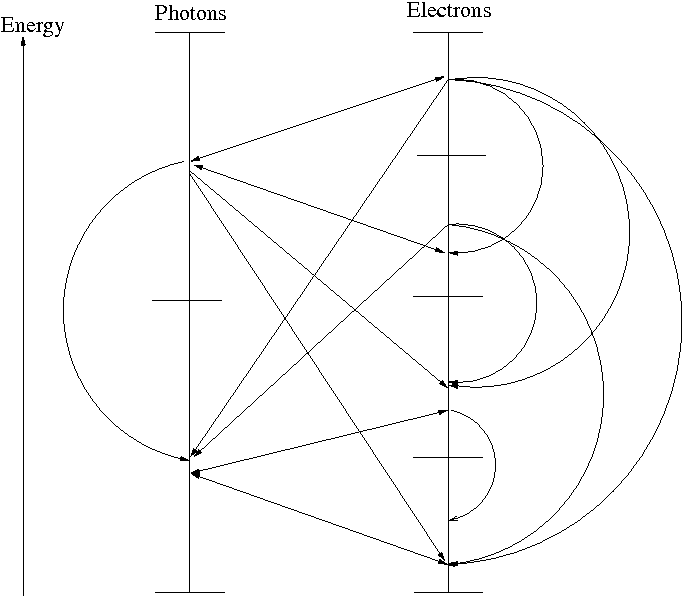
\includegraphics[height=7cm]{group.png}
\caption{Transfer between the different groups}        
\label{joli}
\end{center}
\end{figure}
The pattern of the scattering matrix is as follows :
\begin{equation}
\Sigma =
\begin{pmatrix}
x & 0 & \vline & x & x & 0 & 0\\
x & x & \vline & x & x & x & x\\
\hline     
x & 0 & \vline & x & 0 & 0 & 0\\
x & 0 & \vline & x & x & 0 & 0\\
x & x & \vline & x & x & x & 0\\
x & x & \vline & x & x & x & x\\
\end{pmatrix}
\end{equation}
We can see that there is no upscattering to the first group of photons, the
first and the second group of electrons coming from the second group of
photons, and the third or the fourth group of electrons (see figure
\ref{joli}). Thus, if we reorder the groups using for the first group \hbox{set :} 
photon group 1, electron group 1, electron group 2 and for the second group 
\hbox{set :} photon group 2, electron group 3, electron group 4. The pattern 
of the scattering matrix looks \hbox{like :}
\begin{equation}
\Sigma =
\begin{pmatrix}
x & x & x & \vline & 0 & 0 & 0\\
x & x & 0 & \vline & 0 & 0 & 0\\
x & x & x & \vline & 0 & 0 & 0\\
\hline      
x & x & x & \vline & x & x & x\\
x & x & x & \vline & x & x & 0\\
x & x & x & \vline & x & x & x\\
\end{pmatrix}
\end{equation}
Now, we see that the matrix is block lower triangular and we can solve the
transport problem by solving two problems with only three groups each. 
We can solve the first three groups without solving the last three groups since 
there is no upscattering coming from these. Then, we can solve the last three 
groups, with the first three groups hidden in the source term. Thus, we can 
solve a problem with six groups using the same memory that we would use for 
only three groups. To know how many groups we need to gather from each particle 
in each group set, we can use a simple rule. First, we define the number of 
groups of photons as $n_p$, the number of groups electrons as $n_e$ and the 
greatest common divisor between these two numbers as $gcd$. The number of 
groups of photons to put in a group set is $\frac{n_p}{gcd}$ and the number 
of groups of electrons to put in a group set is $\frac{n_e}{gcd}$. Instead 
of solving one problem of $n$ groups, we can solve $gcd$ problems of 
$\frac{n}{gcd}$ groups.\\
Reordering the groups is also advantageous to decrease the number of
iterations of source iteration or GMRES needed to solve a problem. These two
methods are used to solve the linear system created by the discretized
transport equation of (\ref{solved}).
Below, we compare the number of iterations needed to
solve a problem very similar to the one of the previous section with and
without reordering. The domain is
made of aluminium, we use a $S_{12}$ angular discretization and $P_5$ expansion
for the scattering cross section. We use linear discontinuous finite elements 
for the spatial discretization, there are 1800 cells and we have 15 groups 
of photon and 25 groups of electron. We obtain the following result :
\begin{table}[H]
\begin{center}
\caption{Comparison of the number of iterations with and without group reordering}
\begin{tabular}{|c|c|}
\hline
With reordering & Without reordering\\
\hline
7594 & 7968\\
\hline
\end{tabular}
\end{center}
\end{table}
The saving is about 4.7\% fewer iterations.

At this time, we cannot compare the number of iterations when we reorder the
groups and then split the problem in
subproblems with our code. When we split the problem in subproblems with our
code, we
solve all the groups at the same time. All the groups of a subproblem are
solved simultaneously and therefore, we cannot take full advantage of the
decrease of number of iterations. When we reorder the groups, we mix photon and
electron groups and since the photons converge faster, we need to do some
extra iterations that are useless for the photons but needed for the
electrons. If we split the problems without reordering, the photon groups are
solved together in a few iterations. Because there is no extra iterations to
solve the photon groups, we need fewer iterations if we do not reorder the
groups. We plan to modify our code to take advantage of the reordering.
